\section*{Introduction}
\addcontentsline{toc}{section}{Introduction}
\dots
\newpage
\section{Résumé}

\section{Cadrage}
\subsection{Finalités et importance du projet}
L’analyse tactique dans les sports collectifs connaît une croissance exponentielle grâce aux avancées en vision par ordinateur et en apprentissage automatique (\emph{Machine Learning}). Ces technologies permettent aujourd’hui de comprendre et d’optimiser les stratégies de jeu avec une précision et une profondeur sans précédent.

Le projet \textbf{TactIAque} s’inspire des récents travaux de \textbf{RoboFlow}, une initiative pionnière visant à améliorer les algorithmes d’analyse tactique pour le football. Toutefois, le basketball reste un domaine encore sous-exploré dans ce contexte, offrant une opportunité unique de développement et d’innovation. Ce projet se concentre donc sur le basketball, avec pour objectif de fournir des outils robustes pour l’analyse des tactiques dans ce sport collectif.

En combinant des méthodologies existantes et des innovations spécifiques au basketball, \textbf{TactIAque} vise à combler cette lacune en proposant des solutions adaptées aux exigences de ce sport.
\subsubsection{Hypothèses de lancement}
    \paragraph{Compétences des membres de l'équipe}
    \paragraph{Moyens techniques à disposition}
    \paragraph{Obstacles à lever}
    \paragraph{Analyse SWOT}
    L’analyse SWOT met en évidence les éléments clés influençant la réussite du projet. Voir la figure \ref{tab:swot}
    \begin{table} [!h]
        \centering  
        \begin{tabular}{|p{7cm}|p{7cm}|}  
        \hline  
        \textbf{Forces (Strengths)} & \textbf{Faiblesses (Weaknesses)} \\  
        \hline  
        \begin{itemize}
        \item Disponibilité de modèles performants comme RT-DETR, reconnus pour leur efficacité en détection multi-objets. 
         \item Outils avancés tels que HuggingFace, facilitant le fine-tuning et l’itération rapide. 
         \item Accès à une infrastructure puissante pour l’entraînement (GPU haute performance). 
        \end{itemize}
        & 
        \begin{itemize}
         \item Dépendance critique à une annotation de haute qualité, nécessitant des ressources humaines et financières importantes. 
         \item Complexité des scènes sportives, avec des objets en mouvement rapide et des interactions multiples. 
         \item Risque de sur-ajustement du modèle en raison de la limitation des données annotées. 
        \end{itemize}\\
         \hline  
        \textbf{Opportunités (Opportunities)} & \textbf{Menaces (Threats)} \\  
        \hline  
        \begin{itemize}
            \item Possibilité de générer des résultats innovants et publiables dans des conférences ou journaux scientifiques.   
            \item Intérêt croissant pour l’analyse des sports à l’aide de l’IA, ouvrant des opportunités de collaboration ou de financement.  
            \item Potentiel d’application du modèle à d’autres sports, élargissant les cas d’usage.
        \end{itemize}&
        \begin{itemize}
            \item Risque de données insuffisantes ou de faible diversité, compromettant la généralisation du modèle. 
            \item Problèmes potentiels de droits et d’accès aux vidéos de matches pour constituer la base de données. 
            \item Délais stricts pour livrer les résultats dans le cadre du projet TactIAque. 
        \end{itemize}\\
        \hline  
        \end{tabular}  
        \caption{Matrice SWOT pour la détection des joueurs}  
        \label{tab:swot}
    \end{table} 
\clearpage
\subsection{Contexte/Hypothèses de départ}
\subsubsection{Clients}
\subsubsection{Partenaires}
\subsubsection{Principales fonctions identifiées par le cahier des charges}

\clearpage
\subsection{Objectifs et résultats opérationnels : liste des livrables}
produits, services, documentation
\begin{figure}[!h]
	\begin{center} 
		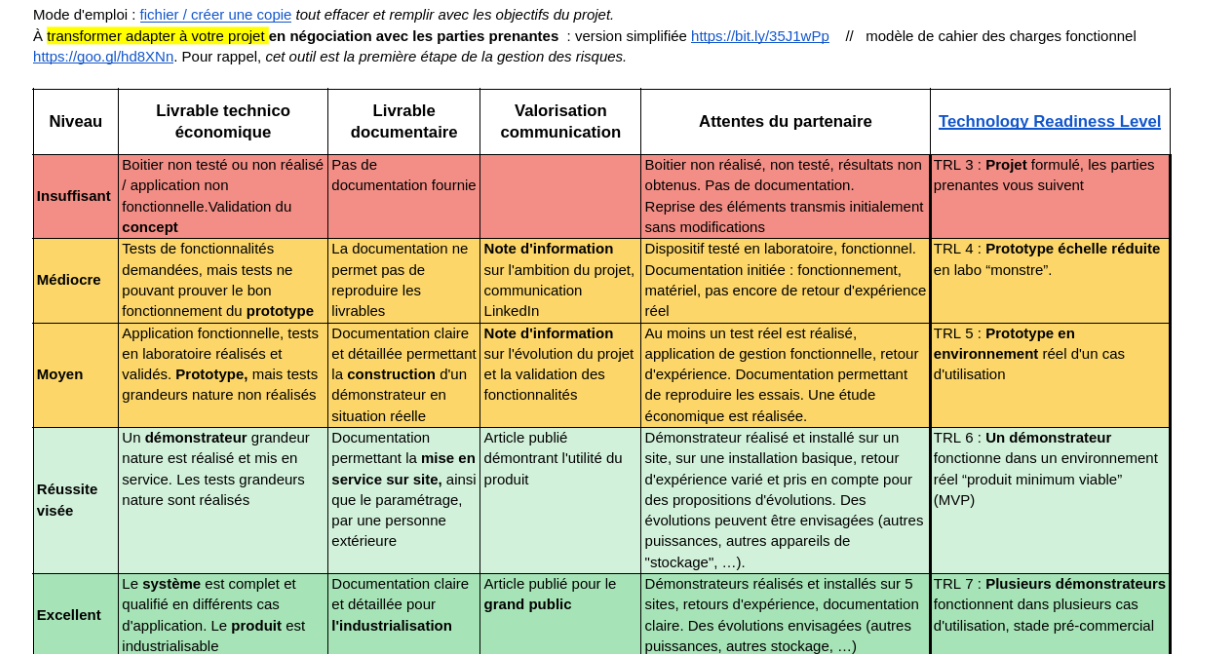
\includegraphics[scale=0.4]{images/modele_plus_exhaustif_matrice_objectifs.png}
		\caption{modèle exhaustif de la matrice des objectifs : https://bit.ly/2IgKrPD}
	\end{center}
\end{figure}
\subsubsection{Critères et indicateurs de succès}
\subsubsection*{Détection et suivi}
\begin{itemize}
    \item \textbf{Précision de détection des joueurs :} Pourcentage de joueurs correctement détectés (objectif : $>$95\%).
    \item \textbf{Précision de l’attribution des équipes :} Exactitude des associations joueur-équipe (objectif : $>$90\%).
    \item \textbf{Fréquence d’actualisation :} Images par seconde (objectif : $\geq$25 FPS).
\end{itemize}

\subsubsection*{Localisation et analyse}
\begin{itemize}
    \item \textbf{Erreur de positionnement :} Distance moyenne entre les positions calculées et les positions réelles des joueurs (objectif : $<$10 cm).
\end{itemize}

\section{Déroulement du projet}
\subsection{Organisation/ ressources, budget}
\subsubsection{Roles et responsabilités, comité de pilotage du projet et budget}
\paragraph{Roles et responsabilités des membres de l'équipe}
\paragraph{Roles et responsabilités des autres parties prenantes}
    \subparagraph{Client}
    \subparagraph{Financeur}
    \subparagraph{\dots}
\paragraph{Comité de pilotage du projet}

\subsubsection{Budget}
\paragraph{Résumé du budget global}
\begin{itemize}
    \item Montant total estimé pour le projet
    \item Source de financement 
    \item Graphique ou tableau pour une vue d'ensemble
\end{itemize}
\paragraph{Répartition temporelle (échéancier budgétaire)}
Comment les dépenses seront réparties sur la durée du projet
\clearpage
\subsection{Jalons : Echéanciers/événements importants}
\begin{table}[!h]
    \centering  
    \begin{tabular}{|p{7cm}|p{7cm}|}  
    \hline  
    \textbf{Jalons} & \textbf{Description}\\
    \hline
    \textbf{Etape 1 }: exigences opérationnelles & Validations des spécifications : cahier des charges techniques\\
    \hline
    \textbf{Etape 2} : \dots & \dots\\
    \hline
    \end{tabular}
\end{table}
\subsection{Risques et opportunités}
\subsubsection{Identification des risques}
\begin{figure}[!h]
	\begin{center}
		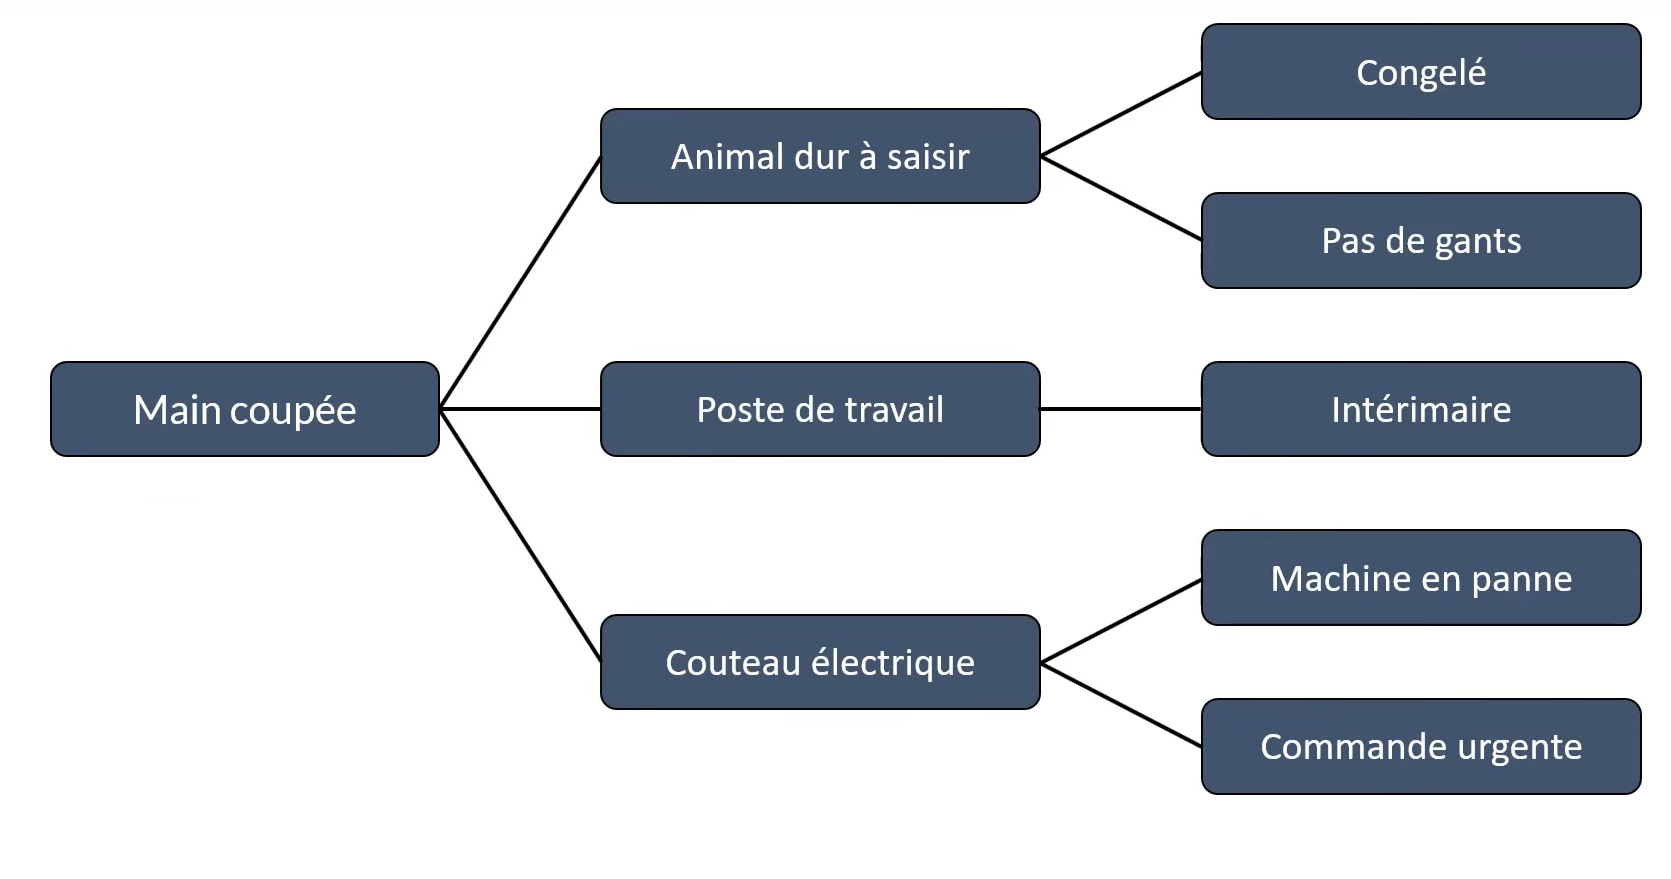
\includegraphics[scale=0.25]{images/arbre_causes.png}
		\caption{Arbre de causes}
		\label{fig:arbre_causes}
	\end{center}
\end{figure}
\subsubsection{Un plan de prévention efficace}
Nous avons un exemple de plan de prévention à la figure \ref{fig:plan_prevention}.
\begin{danger}
	Il ne faut pas oublier de tier le tableau pour mettre en haut les risques prioritaires
\end{danger}
\begin{figure}[!h]
	\begin{center}
		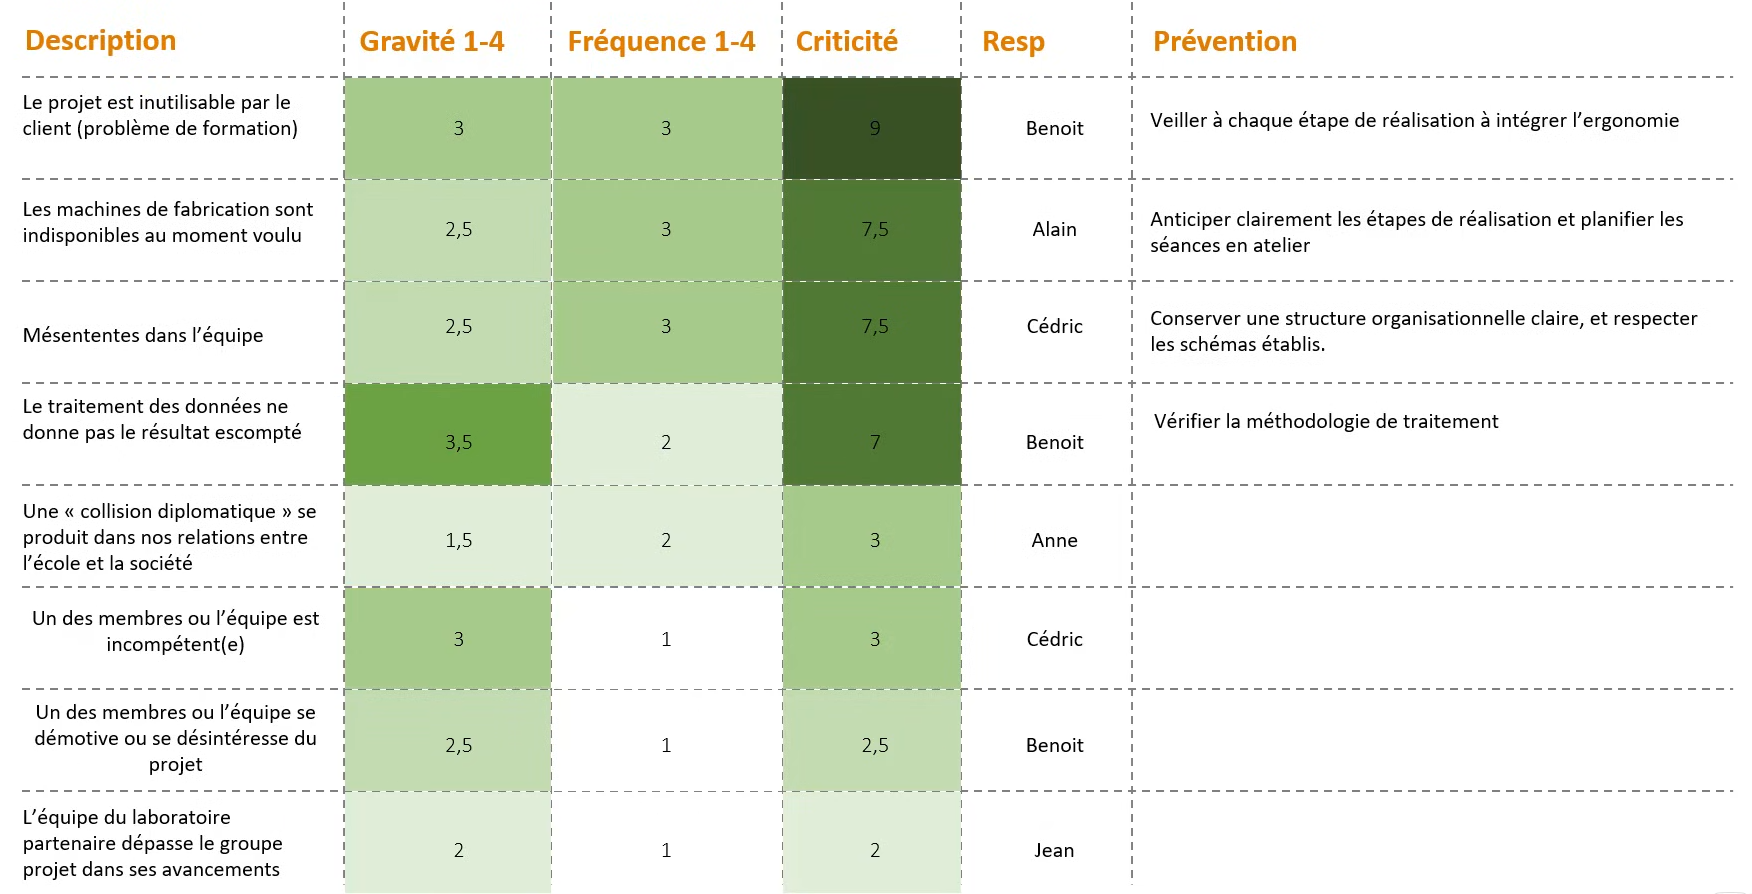
\includegraphics[scale=0.25]{images/plan_prevention.png}
		\caption{Plan de prévention}
		\label{fig:plan_prevention}
	\end{center}
\end{figure}
Sur OpenCV, on peut définir des algorithmes à partir d'un exemple d'annotation pour faire des transformations qui nous aideront pour le suivi de objets.
\clearpage
\section{Cahier des charges techniques : exigences opérationnelles}
\subsection{Parties prenantes}
\begin{itemize}
    \item ENSTA (MOA)
    \item Groupe projet élèves (en tant que MOE)
    \item 
\end{itemize}
\subsection{Exigences}
\subsubsection{Exigences fonctionnelles}
\section*{Exigences Fonctionnelles}
\begin{enumerate}
    \item \textbf{Détection des joueurs et des équipes :}
    \begin{itemize}
        \item Le système doit identifier tous les joueurs visibles dans une vidéo et leur associer une équipe.
        \item Il doit identifier le joueur en possession de la balle avec une précision supérieure à 90\%.
        \item Il doit identifier le ou les arbitres avec une précision supérieure à 90\%.
    \end{itemize}
    
    \item \textbf{Suivi des joueurs :}
    \begin{itemize}
        \item Le système doit suivre les mouvements de chaque joueur sur le terrain en temps réel et enregistrer leurs trajectoires.
        \item La position des joueurs doit être mise à jour à une fréquence d’au moins 25 FPS (images par seconde).
    \end{itemize}
    
    \item \textbf{Localisation des joueurs sur le terrain :}
    \begin{itemize}
        \item Le système doit convertir les positions des joueurs depuis l’espace de la vidéo en coordonnées sur le terrain réel.
        \item Il doit pouvoir gérer des perspectives différentes des caméras et aligner les positions avec un plan du terrain.
    \end{itemize}
    
    \item \textbf{Visualisation des trajectoires :}
    \begin{itemize}
        \item Une interface graphique doit afficher les trajectoires des joueurs sur une représentation schématique du terrain.
        \item La visualisation doit inclure des options de filtrage (par joueur, par équipe, par période de temps).
    \end{itemize}
    
    \item \textbf{Analyse tactique :}
    \begin{itemize}
        \item Le système doit identifier le ou les joueurs pivots avec une précision supérieure à 90\%.
        \item Identifier des patterns tactiques globaux (exemple : formation, stratégies défensives/offensives).
        \item Analyser des situations spécifiques pour prédire des événements comme un tir ou une interception.
    \end{itemize}
\end{enumerate}

\section*{Exigences Non Fonctionnelles}
\begin{enumerate}
    \item \textbf{Performance :}
    \begin{itemize}
        \item Le système doit traiter une vidéo de 10 minutes en moins de 5 minutes.
        \item Pour l’analyse en temps réel, la latence de détection ne doit pas dépasser 100 ms.
    \end{itemize}
    
    \item \textbf{Fiabilité :}
    \begin{itemize}
        \item Le système doit fonctionner avec un taux d’erreur inférieur à 5\% pour la détection des joueurs et des équipes.
    \end{itemize}
    
    \item \textbf{Interopérabilité :}
    \begin{itemize}
        \item Le produit doit être compatible avec plusieurs formats vidéo (MP4, AVI, etc.).
    \end{itemize}
\end{enumerate}
\subsubsection{Vision boite noire du système}
\begin{figure}[!h]
    \begin{center}
        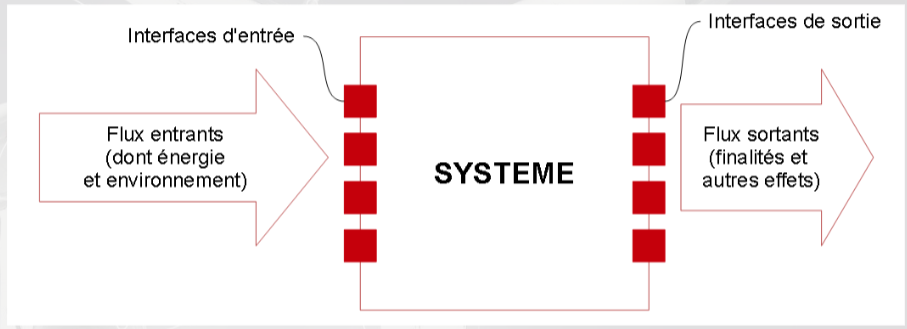
\includegraphics[scale=0.5]{images/boite_noire.png}
        \caption{Vision boite noire du système}
    \end{center}
\end{figure}
\subsubsection{Diagramme FAST}
Description du système en modules fonctionnels (regroupement de fonctions élémentaires) avec leur séquencement (temporel, logique ou conditionnel) et leurs échanges de flux.
\begin{figure}[!h]
    \begin{center}
        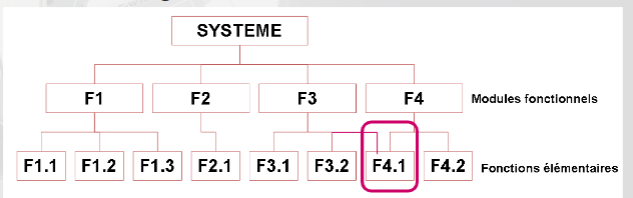
\includegraphics[scale=0.7]{images/fast.png}
        \caption{Diagramme FAST}
    \end{center}
\end{figure}
\begin{figure}[!h]
    \begin{center}
        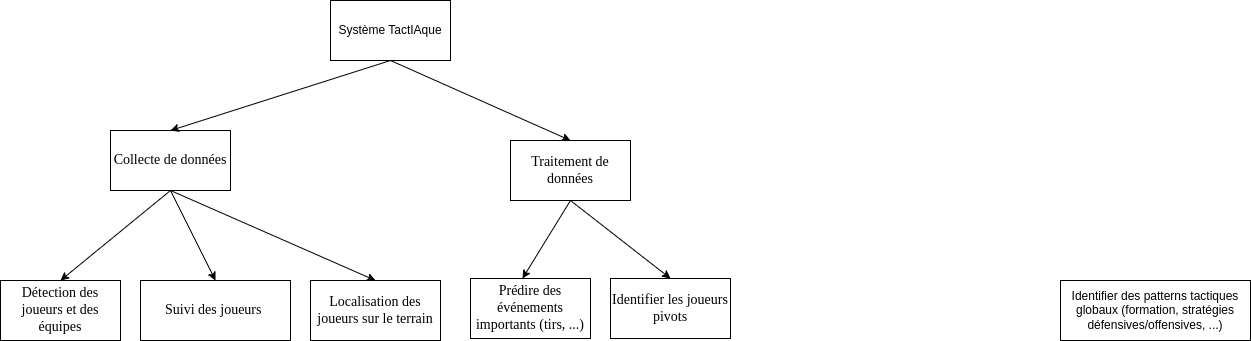
\includegraphics[scale=0.5]{images/tactIAque_fast.png}
        \caption{Diagramme FAST}
    \end{center}
\end{figure}
\subsubsection{Logigramme / chaine fonctionnelle}
A partir des modules fonctionnels et des fonctions élémentaires identifiées dans le diagramme FAST, le logigramme nous permet : 
\begin{itemize}
    \item D'ordonnancer les fonctions entre elles 
    \item D'identifier les interfaces entre les fonctions 
    \item D'identifier (pour les fonctions élémentaires) quel équipement du système supporte la fonction
\end{itemize}
\begin{figure}[!h]
    \begin{center}
        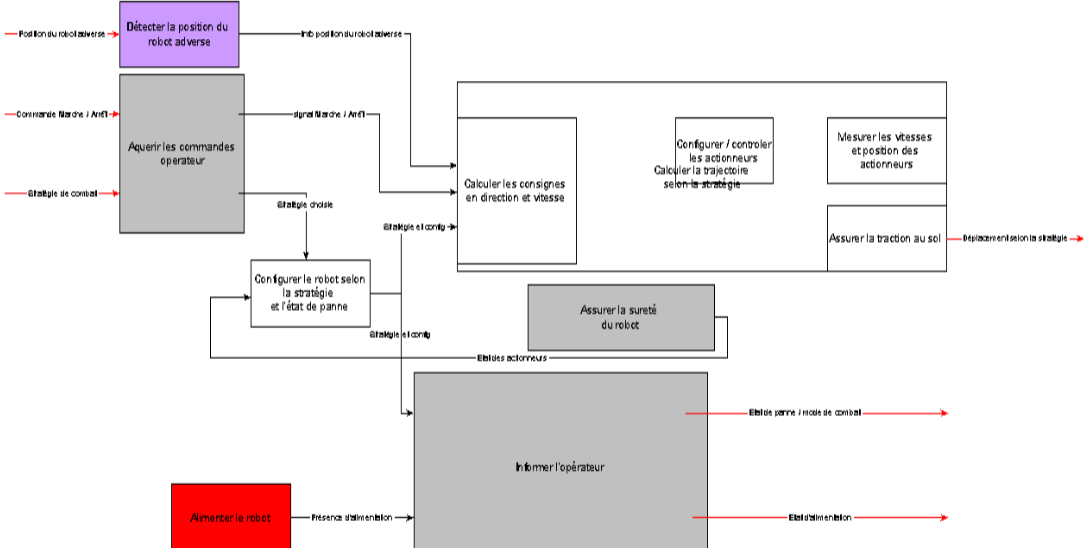
\includegraphics[scale=0.5]{images/logigramme.png}
        \caption{Logigramme}
    \end{center}
    \end{figure}
\subsubsection{Matrice des exigences}
\begin{figure}[!h]
\begin{center}
    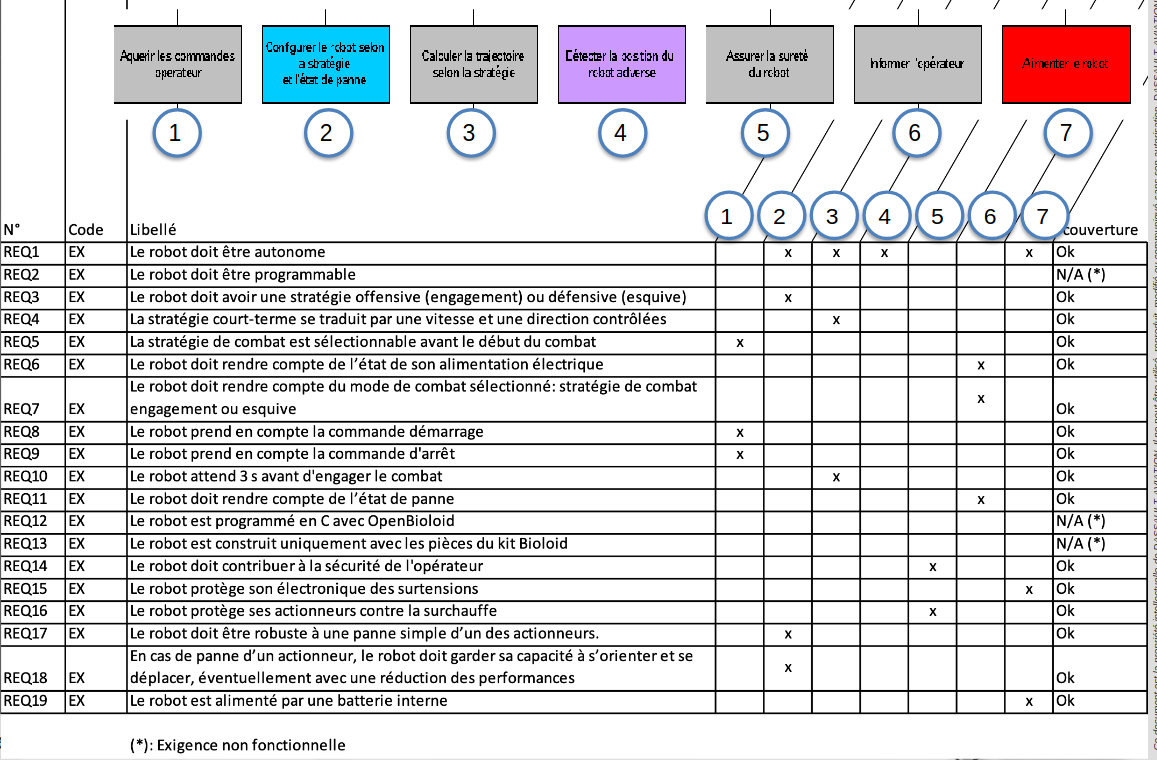
\includegraphics[scale=0.5]{images/matrice_exigences.png}
    \caption{Matrice des exigences}
\end{center}
\end{figure}
\clearpage
\section{Répartition des responsabilités}

\subsection{Lots et responsabilités}
Le \textbf{WBS} est une opération très délicate de séquençage du projet, qui permet de :
\begin{itemize}
	\item Réduire sa complexité pour le maitriser
	\item Préparer son pilotage
\end{itemize}
\paragraph*{Traduire les besoins en Work Packages}
Une fois que le client a défini son projet et que celui ci a été formalisé dans le cahier de charge et la charte de projets, le maitre d'oeuvre doit pouvoir le réaliser. Le défi est de passer d'une logique fonctionnelle au résultat tels qu'ils ont été formalisés dans le cahier de charges et la charte de projet, \textbf{à une logique de travaux}.

On doit convertir le "quoi faire?" en "comment faire?" en déterminant les lots de travail nécessaires pour réaliser chaque fonction.

Cela permet d'obtenir l'organigrame des taches, ce qu'on appelle couramment le \textbf{WBS}(work breakdown structure).\\

\paragraph*{Les lots de travail / Work packages}
Pour chaque tache de travail, on décompose selon un critère donné. Par exemple le métier qui réalise le travail, la localisation du chantier, l'ordre de succession.
Un exemple de WBS à la figure \ref{fig:exemple_wbs}
\begin{sidewaysfigure}[!h]
	\begin{center}
		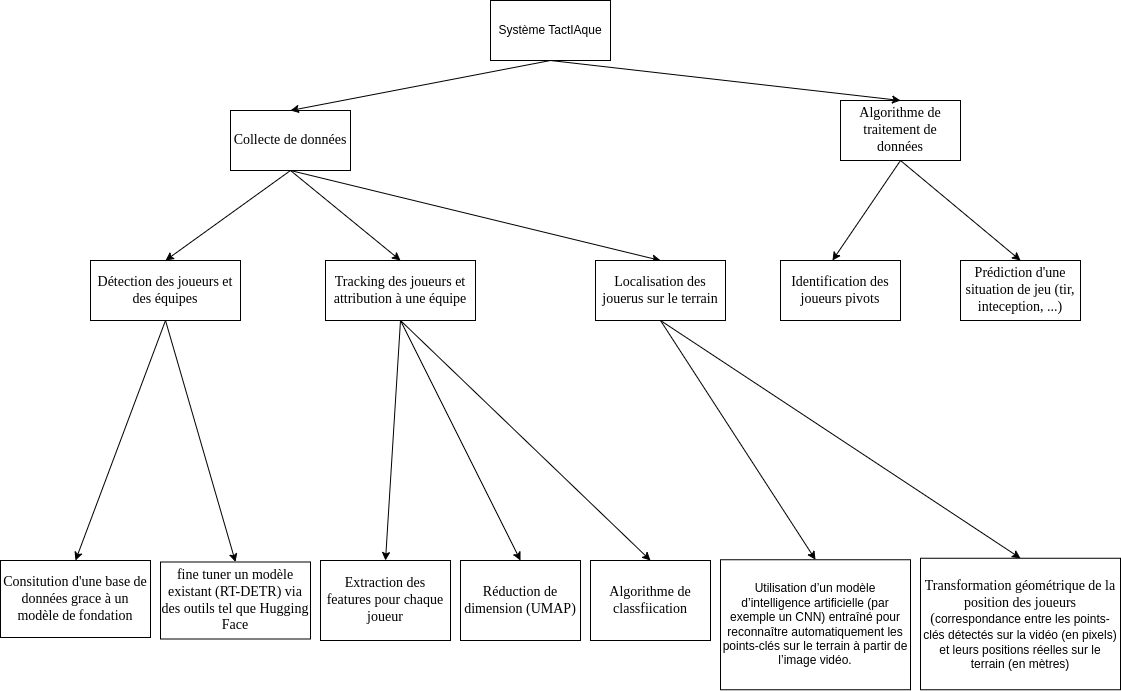
\includegraphics[scale=0.6]{images/tactIAque_wbs.png}
		\caption{exemple WBS}
		\label{fig:exemple_wbs}
	\end{center}
\end{sidewaysfigure}
\begin{enumerate}
    \item Algorithme de collecte de données
\begin{enumerate}
    \item Détection 
    \begin{itemize}
    \item Consittution d'une base de données en utilisant un modèle de fondation 
    \item fine tuner un modèle existant (RT-DETR) en utilisant des outils à l'état de l'art tel que Hugging Face 
    \end{itemize}
    \item Tracking des joueurs et attribution à une équipe 
    \begin{itemize}
        \item Extraction de features (vecteur pour caractériser chaque joueur)
        \item Réduction de dimension (UMAP) 
        \item Algorithme de classification(k plus proches voisins)
    \end{itemize}
    \item Localisation des joueurs sur le terrain 
    \begin{itemize}
        \item Localisation de point clé sur le terrain soit par réseau de neuronne soit par analyse d'image 
        \item Transformation géométrique de la position des joueurs trouvées aux étapes précédentes
    \end{itemize}
\end{enumerate}
\item Algorithme de traitement de données
\begin{itemize}
    \item identification des joueurs pivots 
    \item prédiction d'un situation de jeu (tir, interception,\dots)
\end{itemize}
\end{enumerate}
\subsection{La matrice RACI}
La \textbf{matrice RACI} est la matrice des responsabilités, elle précise et réparti les roles pour chaque lot de travail, ce qui a pour effet d'éviter les erreurs de communication.

La matrice RACI spécifie quatre types de responsabilités : 
\begin{itemize}
	\item Celui qui \textbf{réalise(R)}
	\item Celui qui a l'\textbf{autorité(A)}
	\item La personne qui \textbf{conseille(C)}
	\item Celel qui est \textbf{informée(I)}
\end{itemize}
\paragraph*{Les responsabilités}
Les 4 types de responsabilités :
\begin{itemize}
	\item Les R sont les membres opérationnels, les réalisateurs du lot de travail. C'est eux qui exécutent la tache.
	\item Le A, c'est l'autorité, celui qui doit rendre des comptes. Le A s'organise comme il veut avec les autres intervenants, mais si le travail n'est pas fait, c'est lui qui assume.
	\item Les C sont généralement ceux qui sont consultés avant la réalisation de certaines taches : ce sont des experts qui apportent les conseils pour préaprer et réussir ce lot de travail.
	\item I, ce sont ceux qui doivent etre tenus informés parcequ'ils sont concernées. Mais ils n'exercent pas un role direct : on avance sans attendre de retour de leur part.
\end{itemize}
\begin{sidewaystable}[ht]
\begin{tabular}{|p{1.2cm}|p{1.2cm}|p{1.2cm}|p{1.2cm}|p{1.2cm}|p{1.2cm}|p{1.2cm}|p{1.2cm}|p{1.2cm}|p{1.2cm}|p{1.2cm}|p{1.2cm}|p{1.2cm}|p{1.2cm}|p{1.2cm}|}
    \hline
    & & Gabriel L.
    &Gabriel B.
    &Rodrigo B.
    &Hana Feki
    &Ewerthon M.
    &Rian S.
    &Davy Araujo
    &Yassine B.
    &Nicolas R.
    &Eduardo P.
    &Guilherme G.
    &Cedric D.
    &Gabriel Ba.\\
    \hline
    \multirow{7}{*}{Lot 1} 
          & Lot 1.1 & R & & A & & & & & & & & & &\\
          \cline{2-15}
          & Lot 1.2 & R & & A & & & & & & & & & &\\
          \cline{2-15}
          & Lot 1.3 & R & & A & & & & & & & & & &\\
          \cline{2-15}
          & Lot 1.4 & R & & A & & & & & & & & & &\\
          \cline{2-15}
          & Lot 1.5 & R & & A & & & & & & & & & &\\
          \cline{2-15}
          & Lot 1.6 & R & & A & & & & & & & & & &\\
          \cline{2-15}
          & Lot 1.7 & R & & A & & & & & & & & & &\\
    \hline
    \multirow{2}{*}{Lot 2}
          & Lot 2.1 & R & & A & & & & & & & & & &\\
          \cline{2-15}
          & Lot 2.2 & R & & A & & & & & & & & & &\\
    \hline
\end{tabular}
\caption{Répartition des tâches}
\label{table:repartition}
\end{sidewaystable}
\clearpage
\section{Plannification}
\paragraph*{Séquencement des work packages : diagramme de PERT}
C'est donner pour chaque lot de travail, son ordre de succession.
\begin{sidewaysfigure}[!h]
	\begin{center}
		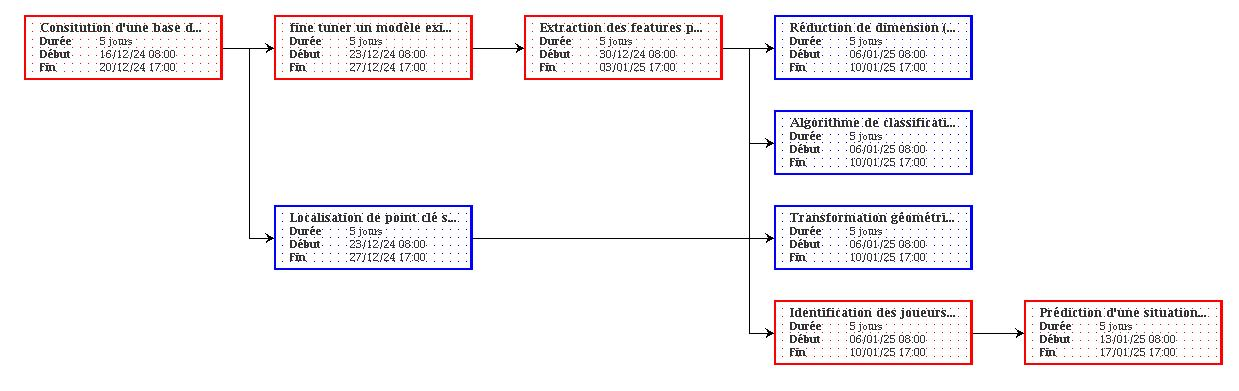
\includegraphics[scale=0.55]{images/TactIAque_pert.jpg}
		\caption{Diagramme de PERT}
	\end{center}
\end{sidewaysfigure}
\paragraph*{Diagramme de Gantt prévisionnel}
\begin{itemize}
	\item Les lots de travail sont représentées par des barres
	\item Les jalons sont représentés par des losanges
	\item Les flêches indiquent les liens entre les tâches
	\item Le chemin critique qui détermine la date de fin du projet
\end{itemize}
\begin{sidewaysfigure}[!h]
	\begin{center}
		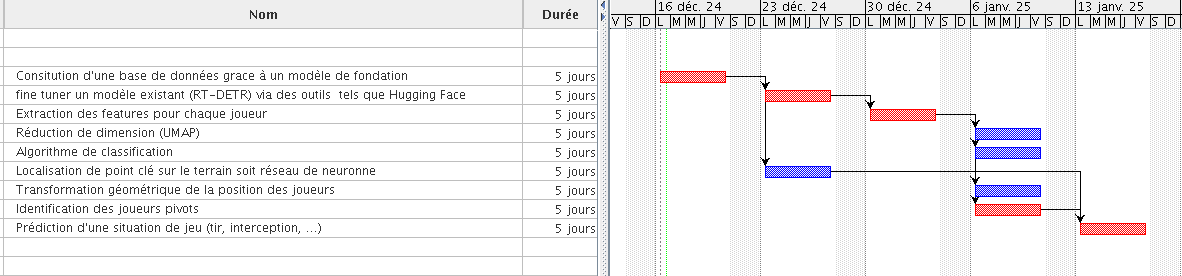
\includegraphics[scale=0.6]{images/tactIAque_gantt.png}
		\caption{Diagramme de Gantt}
    \end{center}
	\end{sidewaysfigure}